The finite element method (FEM) is a numerical technique for solving partial differential equations (PDEs) by discretizing the domain into a collection of finite elements. The basic idea behind the FEM is to represent the solution within each element using a set of basis functions. These basis functions are typically chosen as continuous piecewise polynomials across the element boundaries. By expressing the solution as a linear combination of these basis functions, we can approximate the PDE within each element.

The variational formulation is a vital component of the finite element method. It involves transforming the PDE into an equivalent variational problem, where the goal is finding a solution that minimizes a specific function. This function is typically derived by multiplying the PDE with a test function and integrating it over the domain.

For example, let's consider the heat equation in one dimension:
\[
\partial_t u - \partial_{xx} u = f
\]
To obtain the variational formulation, we multiply the equation by a smooth test function \(v \in C^{\infty}_0(G)\) satisfying \(v(a) = v(b) = 0\), where \(G\) is the domain. 

Then, integrating the heat equation on the whole domain \(G\), we have:
\[
\int_G v \partial_t u\, dx - \int_G v \partial_{xx} u\, dx = \int_G vf\, dx
\]

Now, integrating by parts:
\[
\frac{{d}}{{dt}}\int_G u v \, dx - \left[\partial_x u (t, x) v(x) \right]_{x=a}^{x=b} + \int_G \partial_{x} u \partial_{x} v\, dx = \int_G f v\, dx
\]

Since $v$ is zero on boundaries, the second term on the left-hand side is cancelled (it equals zero).

This equation represents the variational or weak formulation of the heat equation. The goal of the finite element method is to find the solution \(u\) such that \(u(0, x) = u_0(x)\) and, for all smooth test functions \(v \in C^{\infty}_0(G)\), the following equation holds:
\[
\frac{{d}}{{dt}}\int_G u(t, x)v(x)\, dx + \int_G u'(t, x) v'(x)\, dx = \int_G f(t, x) v(x)\, dx
\]

\subsubsubsection{Galerkin Discretization}

Galerkin discretization is a key step in the finite element method (FEM), where we approximate the solution to the partial differential equation (PDE) by projecting it onto a finite-dimensional subspace. Let \(V_N\) be a finite-dimensional subspace of \(H^1_0(G)\). For each \(t \in J\), we approximate \(u(t, \cdot)\) by an element \(u_N(t, \cdot) \in V_N\):

The goal is then to find \(u_N(t, \cdot) \in V_N\) such that \(u_N(0, x) = u_{0,N}(x)\) and for all \(v_N \in V_N\), the following equation holds:

\[
\frac{{d}}{{dt}}\int_G u_N(t, x)v_N(x)\, dx + \int_G u'_{N}(t, x) v'_{N}(x)\, dx = \int_G f(t, x) v_N(x)\, dx
\]

Let \(\{b_j\}_{j=1}^N\) be a basis of \(V_N\). Then, we can express \(u_N(t, x)\) as a linear combination of basis functions:

\[
u_N(t, x) = \sum_{j=1}^N u_{N,j}(t)b_j(x)
\]

where \(\underline{u}_N(t) = (u_{N,1}(t), u_{N,2}(t), \ldots, u_{N,N}(t))^T\) is a vector of unknown functions of \(t\). Similarly, for any \(v_N \in V_N\), \(v_N(x)\) can be written as:

\[
v_N(x) = \sum_{i=1}^N v_{N,i}b_i(x)
\]

where \(v_N = (v_{N,1}, v_{N,2}, \ldots, v_{N,N})^T\) is a vector of coefficients.

\subsubsubsection{Vectorization of the equation}

Hence (we skip the argument \(x\) in \(\int_G\)):

\[
\frac{{d}}{{dt}}\int_G u_N(t)v_N + \int_G u'_{N}(t) v'_{N} = \int_G f(t)v_N, \quad \forall v_N \in V_N
\]

Which can be written as:
\[
\frac{{d}}{{dt}} \bigintssss_G \left(\sum_{j} u_{N,j}(t)b_j \right) \left( \sum_{i} v_{N,i}b_i \right) + \bigintssss_G \left( \sum_{j} u_{N,j}(t)b_{j} \right)' \left( \sum_{i} v_{N,i}b_{i} \right)' = \bigintssss_G f(t) \sum_{i} v_{N,i} b_i
\]

Simplifying further and denoting derivative with respect to time as $\dot{u}$, we have:

\[
\sum_{i} v_{N,i}\left(\sum_{j} \dot{u}_{N,j} \int_G b_j b_i + u_{N,j} \int_G b'_{j} b'_{i} - \int_G f(t) b_i\right) = 0
\]

This equation can be expressed in matrix form as:
\[
\underline{v}_N^T\left(M \underline{\dot{u_N}}(t) + A \underline{u_N} (t) - \underline{f}_N(t)\right) = 0, \quad \forall \underline{v}_N \in R^N
\]

Since it hold for all $\underline{v}_N$, expression in brackets must equal to zero, thus:

\[
M \underline{\dot{u_N}}(t) + A \underline{u_N} (t) = \underline{f}_N(t)
\]

Here \(M\) is the mass matrix with entries \(M_{ij} = \int_G b_i(x) b_j(x)\, dx \), \(A\) is the stiffness matrix with entries \(A_{ij} = \int_G b'_i(x) b'_j(x) \, dx\), \(\underline{f}_N(t)\) is the vector with entries \(f_N(t)_i = \int_G f(t)b_i\), and \(u_N(t)\) is the vector with entries \(u_{N,j}(t)\).

Therefore, we obtain the PDE:
\[
M\underline{\dot{u_N}}(t) + A \underline{u_N}(t) = \underline{f}_N(t),
\]

which is now equal to the initial heat equation \(u_N(t)\) within the finite-dimensional subspace \(V_N\):

\[
\frac{d}{{dt}}(u_N(t), v_N) + a(u_N(t), v_N) = (f(t), v_N), \quad \forall v_N \in V
\]

The Galerkin discretization is a crucial step in the finite element method as it allows us to approximate the PDE solution by solving a system of algebraic equations.

\subsubsubsection{Fully discrete scheme}

We discretize in time. To this end, write \(\underline{u}^m_N := u_N(t^m)\) and \(\underline{f}^m_N := f_N(t^m)\), where the time levels \(t^m\), \(m = 0, \ldots, M\) are as before. Proceeding exactly as in the finite difference method (FDM), the fully discrete scheme reads:

Given \(\underline{u}^0_N = (u_{0,i})^N_{i=1} \in \mathbb{R}^N\), for \(m = 0, \ldots, M-1\) find \(\underline{u}^{m+1}_N \in \mathbb{R}^N\) such that:

\[
M k^{-1} (\underline{u}^{m+1}_N - \underline{u}^m_N) + A(\theta \underline{u}^{m+1}_N + (1-\theta) \underline{u}^m_N) = \theta \underline{f}^{m+1}_N + (1-\theta) \underline{f}^m_N
\]

where \(0 \leq \theta \leq 1\) is the time discretization parameter.

The fully discrete scheme involves solving a system of algebraic equations at each time step, and it provides a numerical approximation of the PDE solution at discrete time instances within the finite-dimensional subspace \(V_N\).

\subsubsubsection{Choice of $V_N$}

The choice of the finite-dimensional subspace $V_N$ is an important aspect of Galerkin discretization. Let's define $B := M + k\theta A$, $C := M - k(1 - \theta)A$, and $\underline{F}^m_N := \theta \underline{f}^{m+1}_N + (1 - \theta) \underline{f}^m_N$. The fully discrete scheme can be written as:

\[
B \underline{u}^{m+1}_N = C \underline{u}^m_N + k \underline{F}^m_N, \quad m = 0, \ldots, M-1.
\]

To choose the space $V_N$, a common and relatively simple choice is to consider the space of piecewise linear, continuous functions. Let $\mathcal{T} := \{a = x_0 < x_1 < \ldots < x_{N+1} = b\}$ be an equidistant mesh on $G$ with $K_i := (x_{i-1}, x_i)$ (as before). We can set the following:

\[
V_N = S^1_0 := \left\{u \in C^0(G): u|_{K_i} \text{ is affine linear on } K_i \in \mathcal{T}\right\}.
\]

It's worth noting that the dimension of $V_N$ is $N$. Choosing piecewise linear functions ensures the simplicity of the basis functions and allows for a straightforward implementation of the finite element method.

A basis $\{b_i\}_{i=1}^N$ of $V_N$ is given by the so-called hat functions $b_i: [a, b] \rightarrow \mathbb{R}_{\geq 0}$, where $b_i(x) = \max\{0, 1 - h^{-1}|x - x_i|\}$ for $i = 1, \ldots, N$. 

The hat functions are defined over the interval $[a, b]$ and have a triangular shape. They take the value of 1 at the centre point $x_i$ of their corresponding subinterval $K_i$ and decrease linearly to zero as we move away from $x_i$. These basis functions capture the local behaviour of the solution within each subinterval.

For example, with equidistant mesh points $a = x_0, x_1, \ldots, x_{N+1} = b$, the basis functions are illustrated as follows:

Here is an illustration of the hat functions for equidistant mesh points:

\begin{figure}[ht]
  \centering
  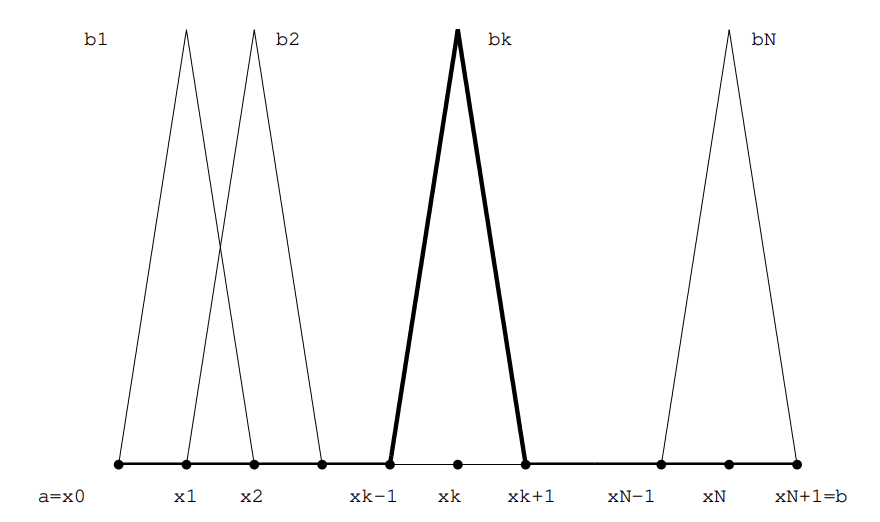
\includegraphics[width=0.6\textwidth]{pdes/fig/hat_functions.png}
  \caption{Illustration of Hat Functions}
\end{figure}

Using this basis, we can calculate the mass and stiffness matrices $M$ and $A$. For equidistant mesh points, we find:

\[
M = \frac{h}{6} \operatorname{tridiag}(1, 4, 1), \quad A = \frac{1}{h} \operatorname{tridiag}(-1, 2, -1).
\]

The mass matrix $M$ and stiffness matrix $A$ are tridiagonal matrices, where the tridiagonal structure arises from the local support of the hat functions and the properties of the integrals involved in their computation.